% ==============================================================================
% TCC - Nome do Aluno
% Capítulo 4 - Projeto Arquitetural e Implementação
% ==============================================================================
\chapter{Projeto Arquitetural e Implementação}
\label{sec-projeto}

Texto

\section{Exibição do Sistema}
\label{sec-projeto-exibicao-sistema}

O sistema possui um controle segurança através da autenticação de usuários, não sendo possível acessar o conteúdo das páginas modificando a URL (\textit{Uniform Resource Locator}) do navegador utilizado. Para ter acesso ao sistema, o usuário deve fornecer o login e a senha que são cadastrados pelos administradores do sistema. Na Figura \ref{fig-projeto-login} é possível visualizar a tela de login.   

\begin{figure}[h]
	\centering
	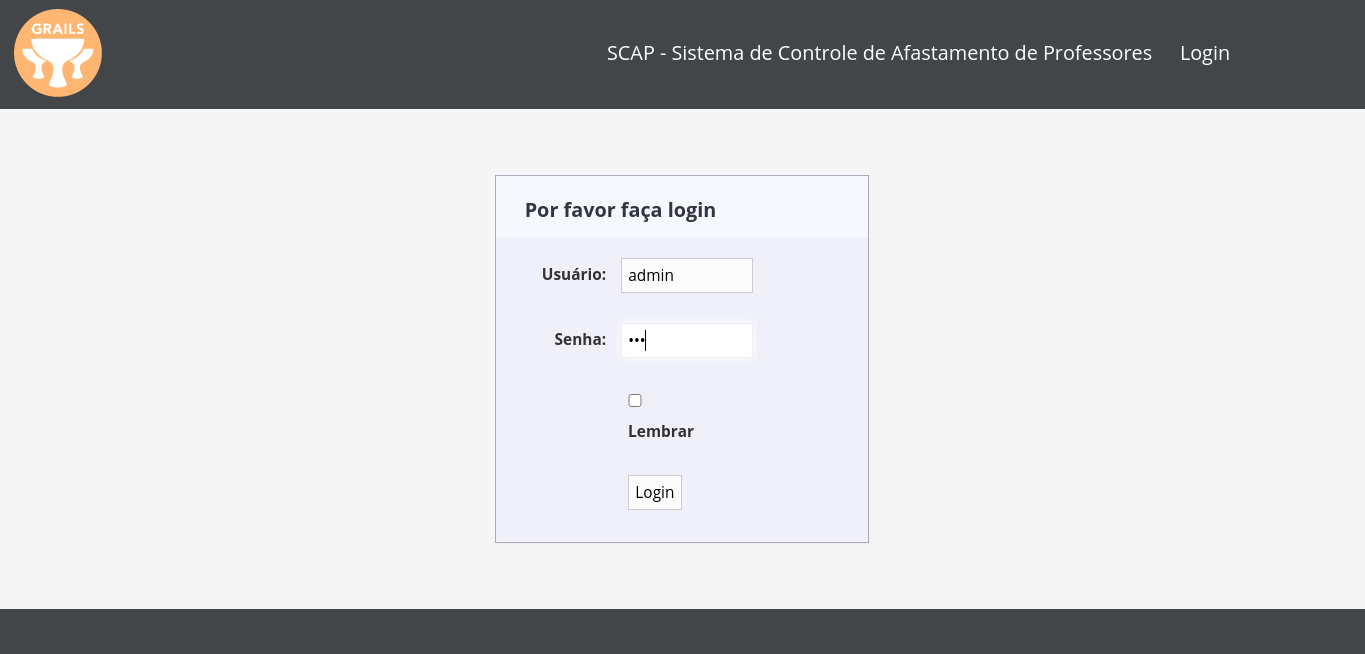
\includegraphics[scale=0.33]{figuras/fig-projeto-login} 
	\caption{Tela de Login do SCAP.}
	\label{fig-projeto-login}
\end{figure}

Por meio de regras de permissão, cada usuário visualiza a tela inicial de uma maneira modificada. Os secretários possuem a regra de permissão de administrador, pois são responsáveis pelo controle da maioria das funcionalidades. Já os professores possuem a regra de permissão de usuário, podendo visualizar as funcionalidades correspondentes ao seu cargo. O professor que se tornar chefe ou subchefe do departamento, pode visualizar todas as funcionalidades referentes aos professores e ainda pode cadastrar relatores para afastamentos internacionais. A Figura \ref{fig-projeto-usuario-secretario} demonstra um usuário secretário que possui a regra de permissão de administrador. Na parte inferior da página do sistema, ficam localizados os botões chamados de controladores. Através deles é possível realizar as ações disponíveis por cada funcionalidade, como a realização de cadastramentos e as suas devidas associações. 

\begin{figure}[h]
	\centering
	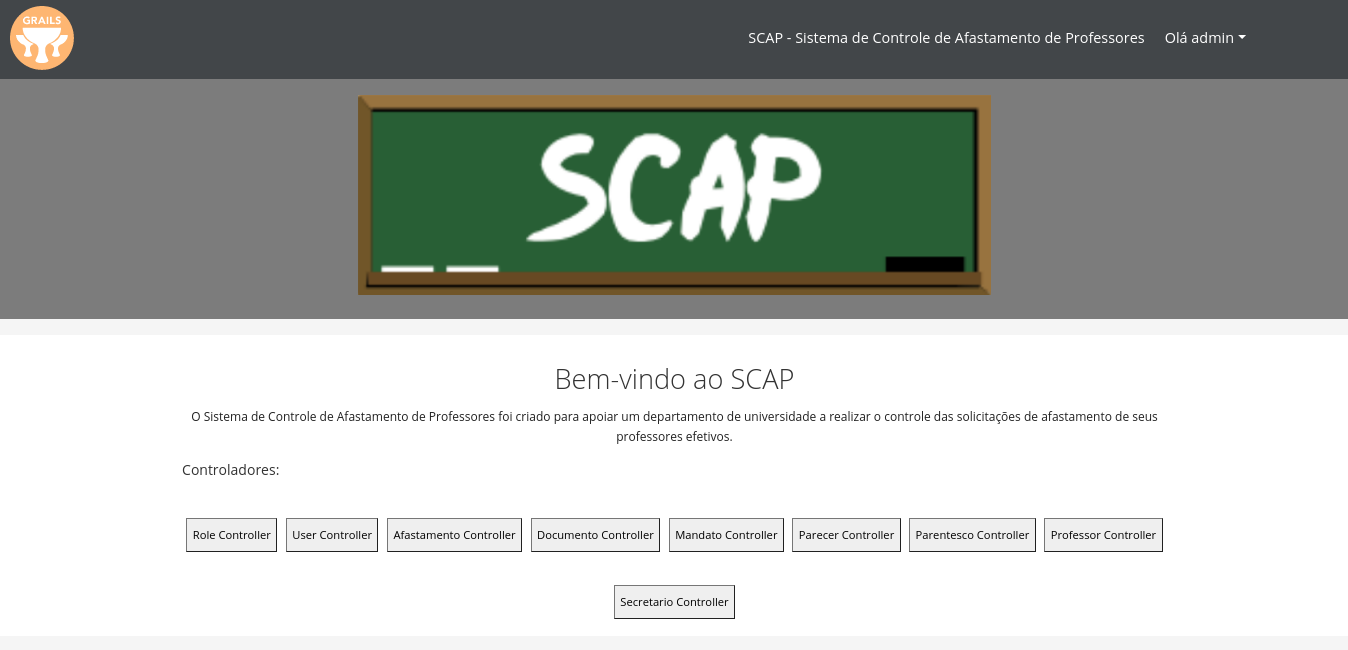
\includegraphics[scale=0.33]{figuras/fig-projeto-usuario-secretario} 
	\caption{Tela Inicial do Usuário Secretário do SCAP.}
	\label{fig-projeto-usuario-secretario}
\end{figure}

Ao clicar no botão ``Professor Controller'', o usuário secretário é redirecionado para a página de cadastramento de professores, pois cabe a ele cadastrar todos os professores e os parentescos entre eles. Para cadastrar os parentescos, o botão ``Parentesco Controller'' deve ser acionado, sendo necessário informar se o parentesco é sanguíneo ou matrimonial. As Figuras \ref{fig-projeto-cadastrar-professor} e \ref{fig-projeto-cadastrar-parentesco} demonstram essas funcionalidades.

\begin{figure}[h]
	\centering
	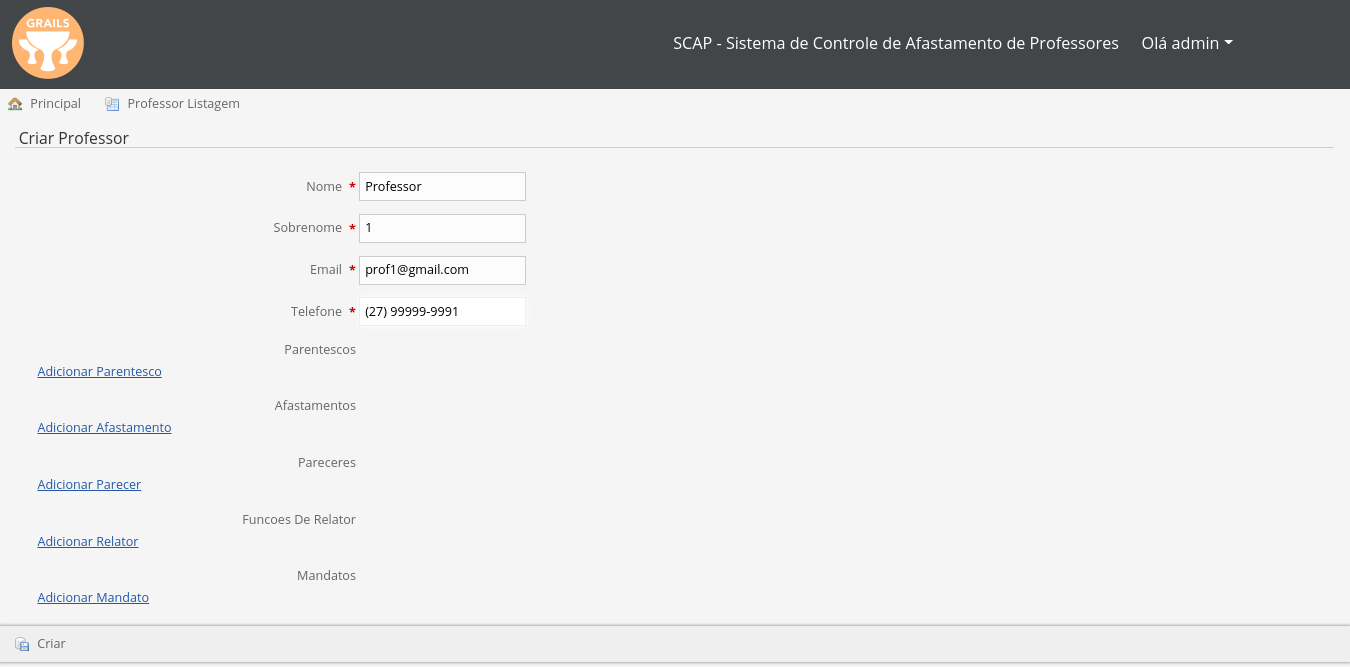
\includegraphics[scale=0.33]{figuras/fig-projeto-cadastrar-professor} 
	\caption{Tela Cadastrar Professor do SCAP.}
	\label{fig-projeto-cadastrar-professor}
\end{figure}

\begin{figure}[h]
	\centering
	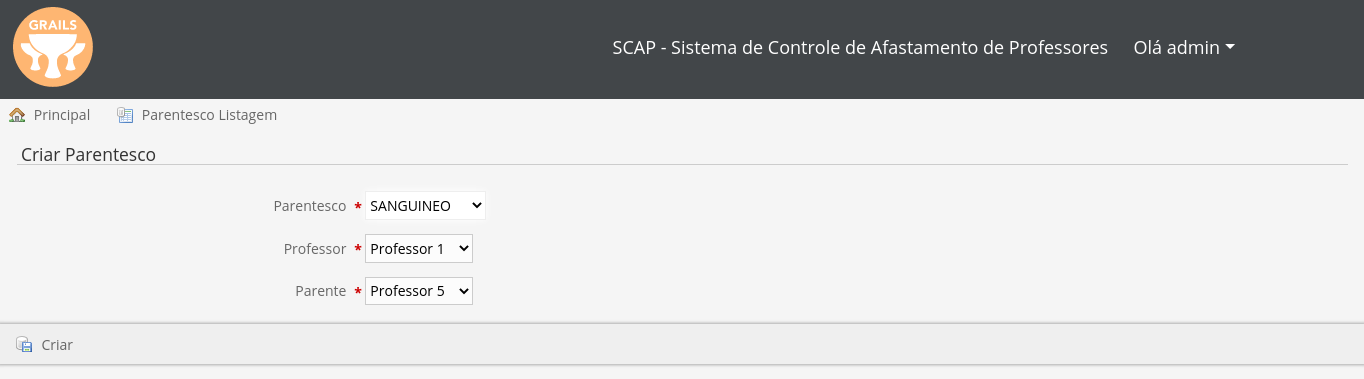
\includegraphics[scale=0.33]{figuras/fig-projeto-cadastrar-parentesco} 
	\caption{Tela Cadastrar Parentesco do SCAP.}
	\label{fig-projeto-cadastrar-parentesco}
\end{figure}

O usuário secretário também tem a responsabilidade de realizar o cadastramento do mandato referente ao chefe ou subchefe do departamento. Para aplicar esta ação, é necessário utilizar o botão ``Mandato Controller'', onde o secretário será redirecionado para a página de cadastro, sendo possível informar o período referente ao mandato e também selecionar o professor na lista de professores cadastrados. Este cadastramento pode ser visualizado através da Figura \ref{fig-projeto-cadastrar-mandato}. 

\begin{figure}[h]
	\centering
	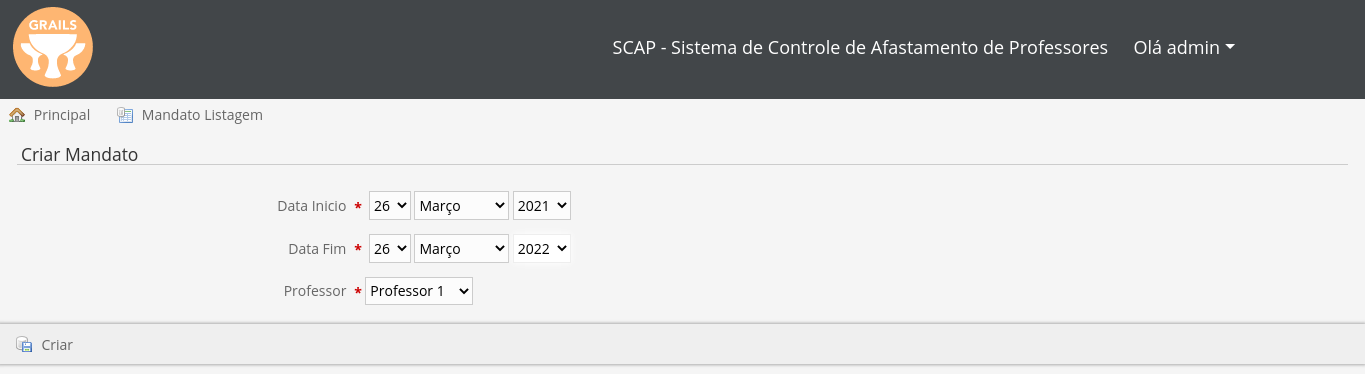
\includegraphics[scale=0.33]{figuras/fig-projeto-cadastrar-mandato} 
	\caption{Tela Cadastrar Mandato do Chefe de Departamento do SCAP.}
	\label{fig-projeto-cadastrar-mandato}
\end{figure}

Após o secretário realizar o cadastramento dos professores, o cadastramento dos parentescos e o cadastramento do mandato referente ao chefe ou subchefe do departamento, os professores recebem o acesso ao sistema. Por possuírem a regra de permissão de usuário, os professores visualizam a tela inicial com as funcionalidades reduzidas. A tela inicial do usuário professor pode ser visualizada através da Figura \ref{fig-projeto-usuario-professor}. 

\begin{figure}[h]
	\centering
	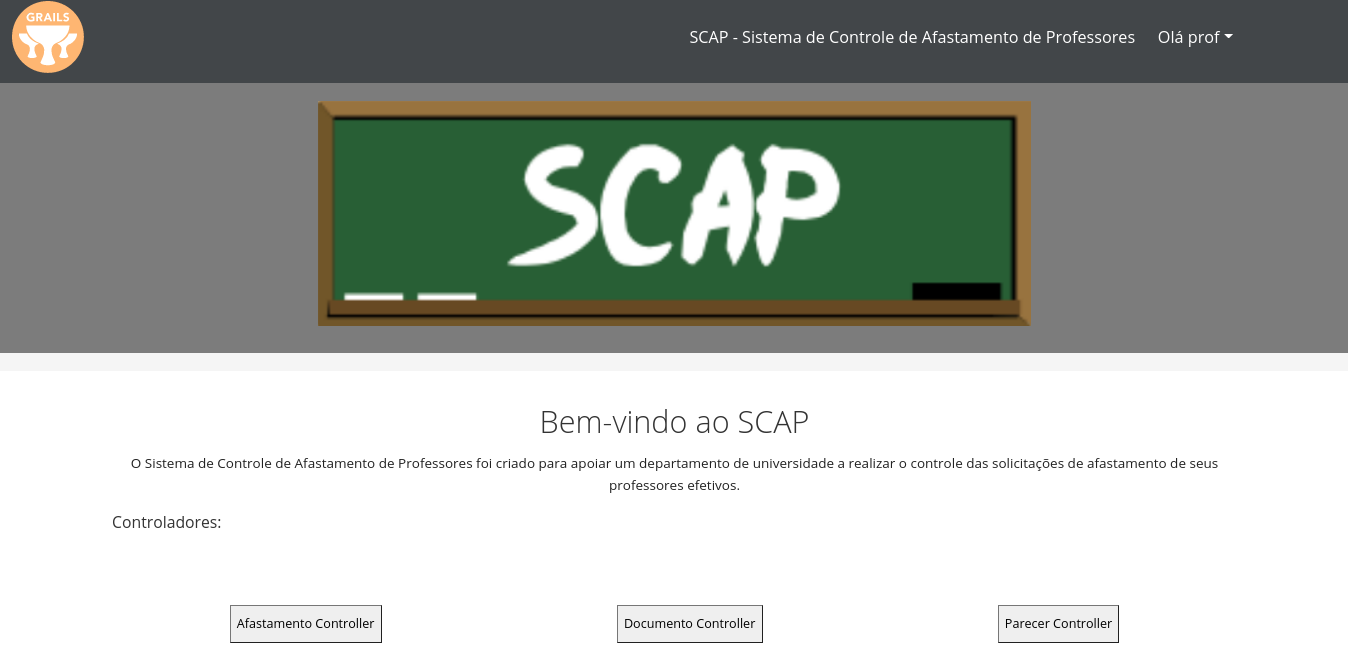
\includegraphics[scale=0.33]{figuras/fig-projeto-usuario-professor} 
	\caption{Tela Inicial do Usuário Professor do SCAP.}
	\label{fig-projeto-usuario-professor}
\end{figure}

A Figura \ref{fig-projeto-cadastrar-afastamento} demonstra a principal funcionalidade do sistema. Ao clicar no botão ``Afastamento Controller'' o professor pode preencher todas as informações necessárias para realizar uma solicitação de afastamento, iniciando todo o processo para que as tramitações sejam aplicadas. Através do botão ``Documento Controller'', é possível cadastrar documentos para que eles sejam associados ao afastamento. Está funcionalidade é demonstrada por meio da Figura \ref{fig-projeto-cadastrar-documento}.   

\begin{figure}[h]
	\centering
	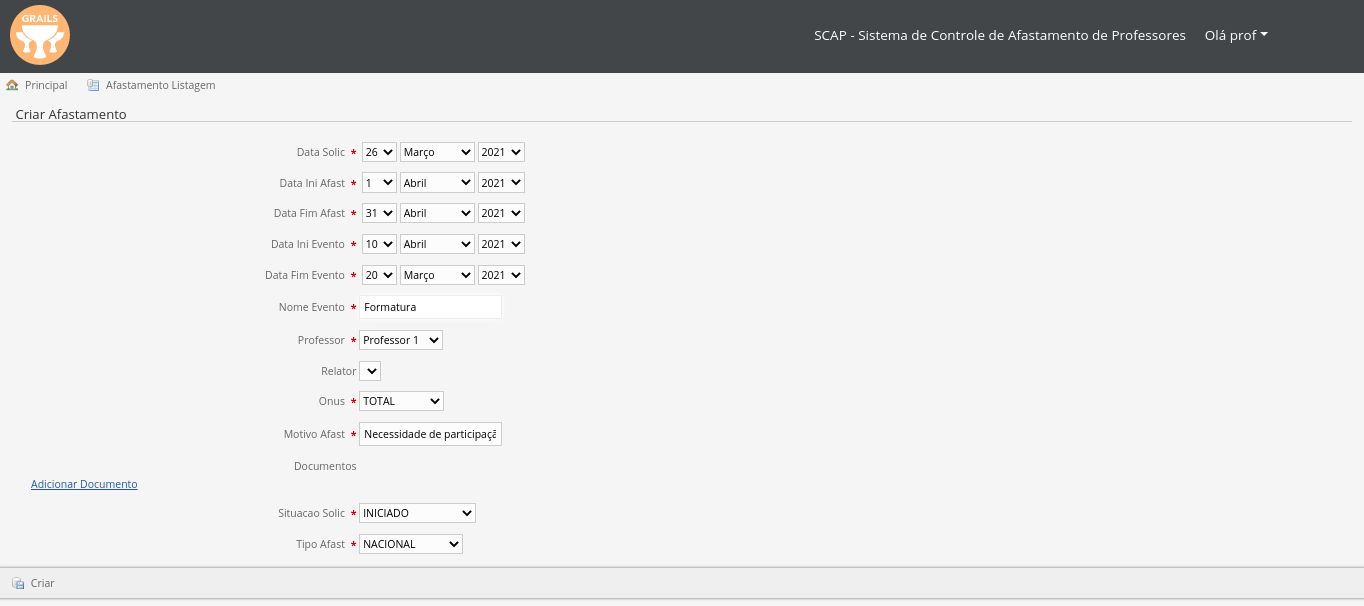
\includegraphics[scale=0.33]{figuras/fig-projeto-cadastrar-afastamento} 
	\caption{Tela Cadastrar Afastamento do SCAP.}
	\label{fig-projeto-cadastrar-afastamento}
\end{figure}

\begin{figure}[h]
	\centering
	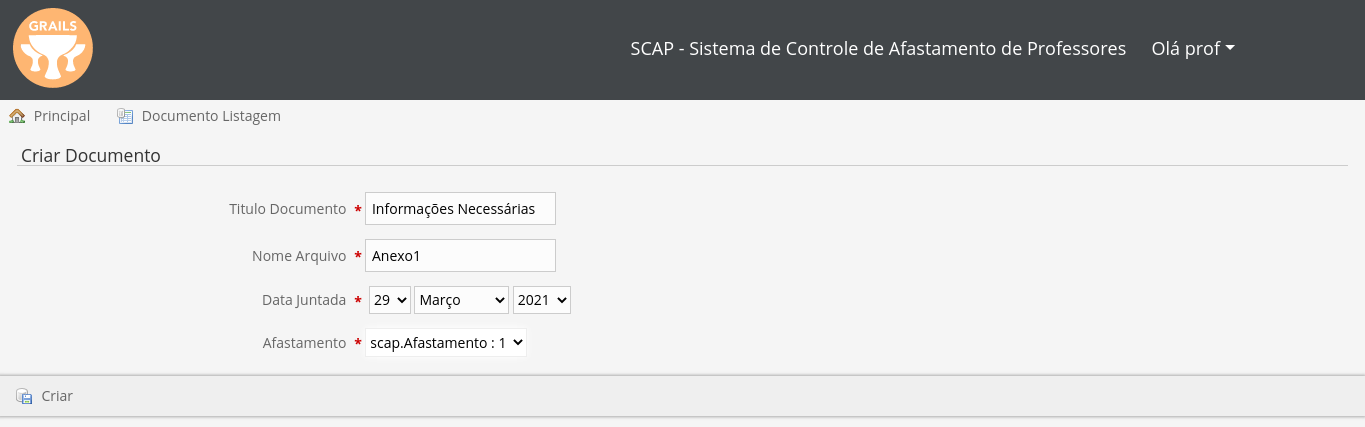
\includegraphics[scale=0.33]{figuras/fig-projeto-cadastrar-documento} 
	\caption{Tela Cadastrar Documento de um Afastamento do SCAP.}
	\label{fig-projeto-cadastrar-documento}
\end{figure}

Se existir uma solicitação de afastamento para um evento internacional, o chefe do departamento pode utilizar o botão ``Relator Controller'' para cadastrar um relator, como demonstra a Figura \ref{fig-projeto-cadastrar-relator}. 

\begin{figure}[h]
	\centering
	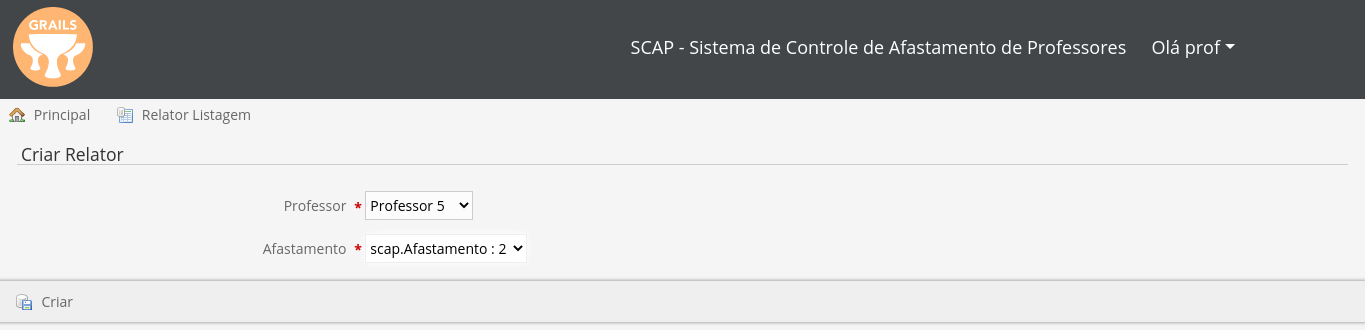
\includegraphics[scale=0.33]{figuras/fig-projeto-cadastrar-relator} 
	\caption{Tela Cadastrar Relator de um Afastamento do SCAP.}
	\label{fig-projeto-cadastrar-relator}
\end{figure}

O cadastro de um parecer é exemplificado pela Figura \ref{fig-projeto-cadastrar-parecer}. Utilizando o botão ``Parecer Controller'', o professor que foi cadastrado pelo chefe do departamento como sendo relator de uma solicitação de afastamento internacional, pode preencher as informações justificando o motivo da sua decisão. 

\begin{figure}[h]
	\centering
	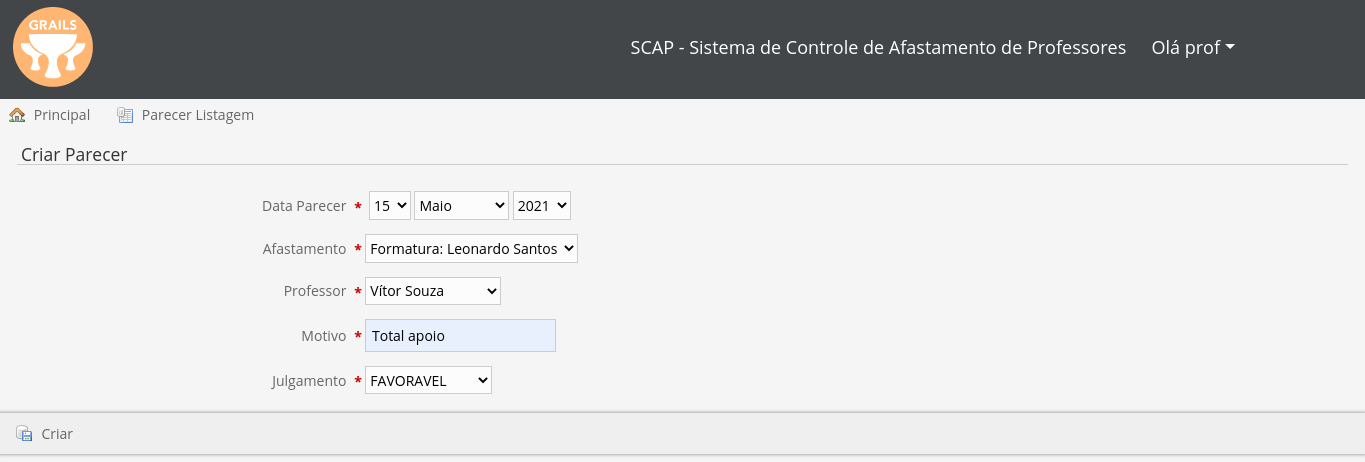
\includegraphics[scale=0.33]{figuras/fig-projeto-cadastrar-parecer} 
	\caption{Tela Cadastrar Parecer de um Afastamento do SCAP.}
	\label{fig-projeto-cadastrar-parecer}
\end{figure}

Todos os usuários do sistema podem realizar consultas para obterem informações sobre uma solicitação de afastamento. É possível visualizar uma lista com todos os afastamentos cadastrados no sistema e também obter detalhes de um afastamento específico. A Figura \ref{fig-projeto-listar-afastamentos} apresenta a lista contendo todos os afastamentos e a Figura \ref{fig-projeto-ver-afastamento} exibe os detalhes do afastamento selecionado.  

\begin{figure}[h]
	\centering
	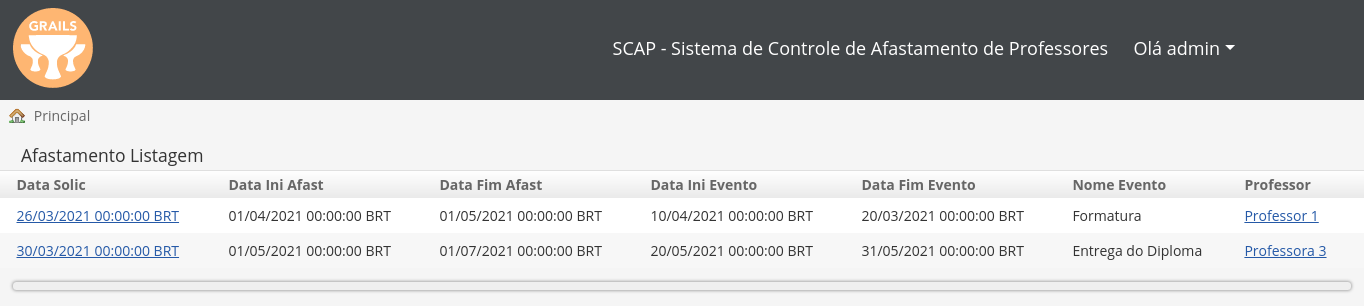
\includegraphics[scale=0.33]{figuras/fig-projeto-listar-afastamentos} 
	\caption{Tela Listar Afastamentos do SCAP.}
	\label{fig-projeto-listar-afastamentos}
\end{figure}

\begin{figure}[h]
	\centering
	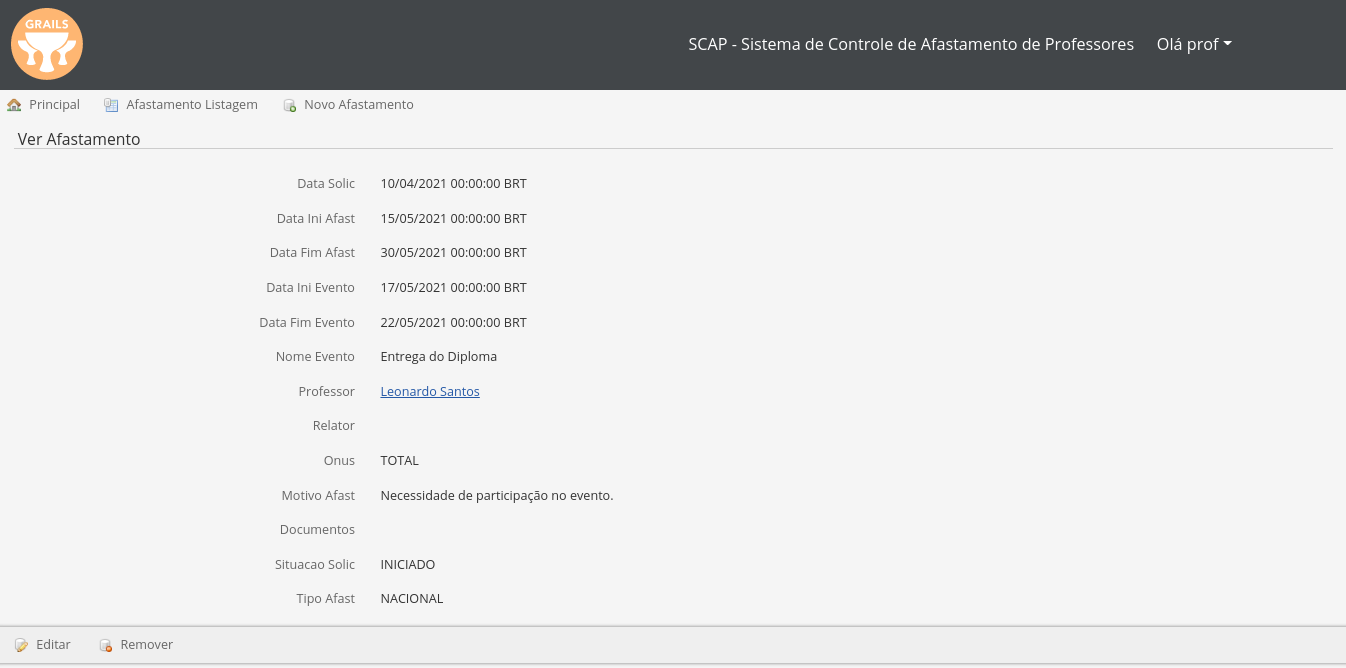
\includegraphics[scale=0.33]{figuras/fig-projeto-ver-afastamento} 
	\caption{Tela Visualizar Afastamento do SCAP.}
	\label{fig-projeto-ver-afastamento}
\end{figure}

A Figura \ref{fig-projeto-listar-professores} demonstra mais uma funcionalidade disponível para o usuário secretário. Para melhorar o controle, é possível visualizar uma lista contendo todos os professores cadastrados, assim como os seus respectivos parentescos. Além disso, é possível saber de todas as solicitações de afastamentos realizadas por cada professor e se ele realizou algum parecer.  

\begin{figure}[h]
	\centering
	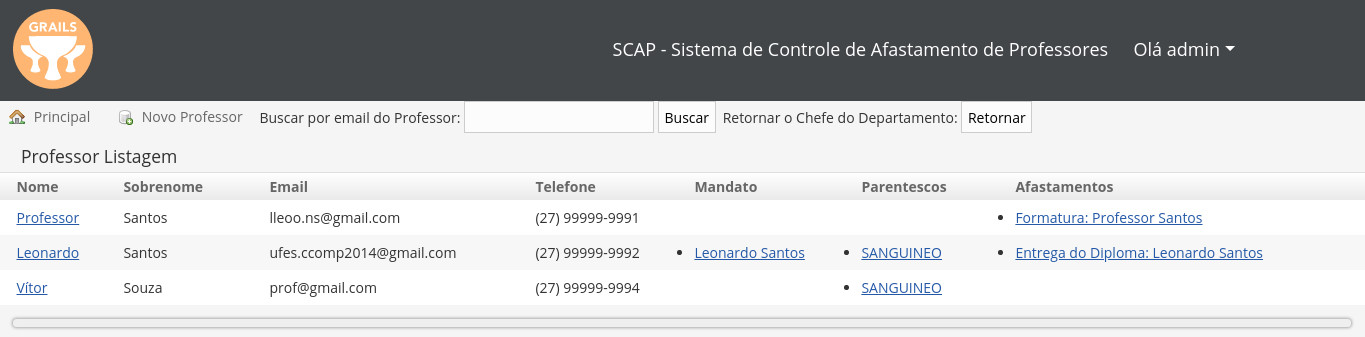
\includegraphics[scale=0.33]{figuras/fig-projeto-listar-professores} 
	\caption{Tela Listar Professores do SCAP.}
	\label{fig-projeto-listar-professores}
\end{figure}

Após as tramitações de um afastamento serem realizada, o usuário secretário deve efetuar uma atualização no afastamento cadastrado, fazendo uma modificação no status do mesmo. Para isso, ele deve editar o afastamento, mudando o campo ``Situacao Solic'' para ``Arquivado''. Por fim, a Figura \ref{fig-projeto-editar-afastamento} exemplifica esta ação.

\begin{figure}[h]
	\centering
	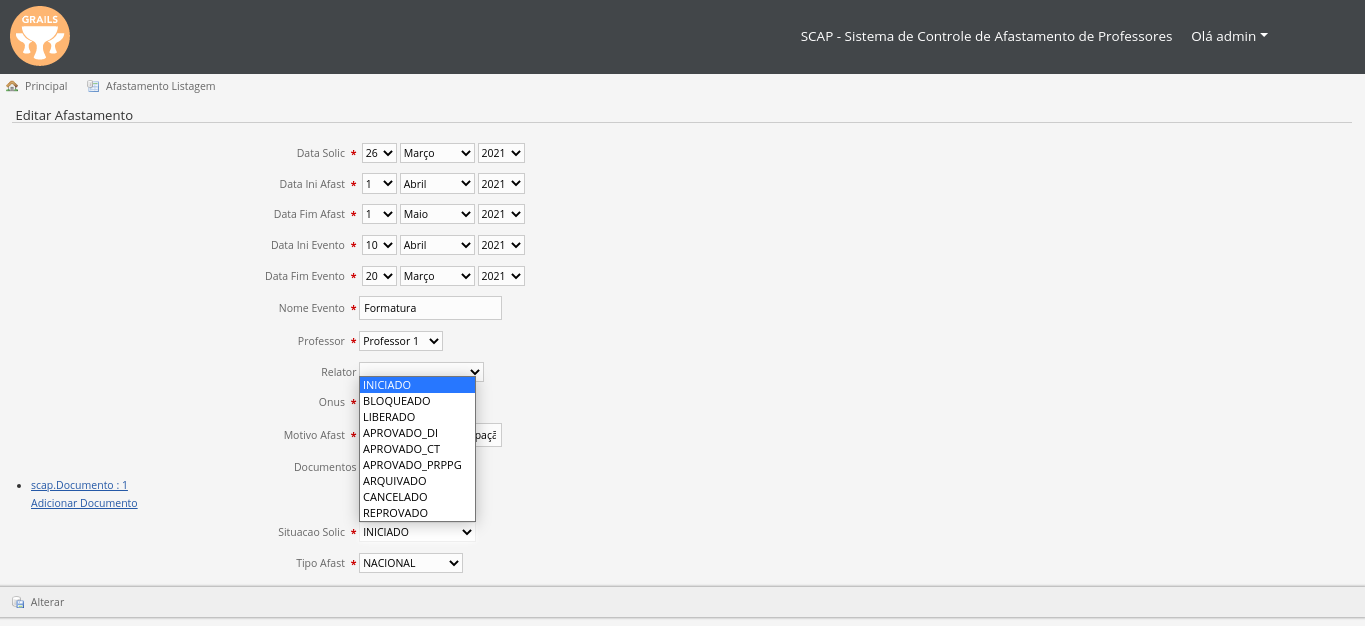
\includegraphics[scale=0.33]{figuras/fig-projeto-editar-afastamento} 
	\caption{Tela Editar Afastamento do SCAP.}
	\label{fig-projeto-editar-afastamento}
\end{figure}

